\documentclass[journal]{IEEEtran}
\usepackage{blindtext}
\let\labelindent\relax
\usepackage[inline]{enumitem}
\usepackage{graphicx}
\usepackage[acronym,toc,shortcuts]{glossaries}
\usepackage{subcaption}
\usepackage[bookmarksopen, bookmarksdepth=2, breaklinks=true]{hyperref}
\usepackage[official]{eurosym}
\usepackage{listings}
\usepackage{multicol}

% *** GRAPHICS RELATED PACKAGES ***
%
\ifCLASSINFOpdf
\else
\fi


\newacronym{ki}{KI}{Künstliche Intelligenz}
\newacronym{gpu}{GPU}{Graphics Processing Unit}
\newacronym{bair}{BAIR}{Berkley AI Research}
\newacronym{cpu}{CPU}{Central Processing Unit}
\newacronym{api}{API}{Application Programming Interface}
\newacronym{cntk}{CNTK}{Microsoft Cognitive Toolkit}
\newacronym{aws}{AWS}{Amazon Web Services}
\newacronym{dsstne}{DSSTNE}{Deep Scalable Sparse Tensor Network Engine}
\newacronym{dl4j}{DL4J}{Deeplearning4j}
\newacronym{ftp}{FTP}{File Transfer Protocol}

\hyphenation{op-tical net-works semi-conduc-tor}

\newcommand{\tab}[1]{\hspace{.2\textwidth}\rlap{#1}}

\begin{document}
\title{Distributed Tensorflow}

\author{\begin{center}
 Michael Zipperle \\ 
 \textit{259564} \\
 Hochschule Furtwangen \\
 Michael.Zipperle@hs-furtwangen.de \\
\end{center}}%
        
% The paper headers
\markboth{Hochschule Furtwangen - Internet of Things, Juli 2018}{}

% make the title area
\maketitle


\begin{abstract}
%\boldmath
Der Einsatz einer \ac{ki} hat in den letzten Jahren stark zugenommen. Einerseits werden die Technologien immer ausgereifter und Big-Player wie Amazon, Microsoft, Facebook und Google treiben die Forschung in diesem Bereich stark voran. Anderseits ermöglichen die Fortschritte in Hardware wie \acs{cpu} und \acs{gpu}, dass diese Technologien optimal eingesetzt werden können. Eine der Hauptherausforderungen stellt die Performance dar, da komplexe neuronale Netzen noch immer eine relativ hohe Trainingszeit von mehreren Stunden oder sogar Tagen benötigen. Dieser Artikel untersucht aktuelle Frameworks, mit denen eine \ac{ki} umgesetzt werden kann. Dabei wird das Framework TensorFlow von Google im Detail betrachtet. Es wird aufgezeigt, wie durch eine verteilte Umgebung über mehrere Instanzen die Performance deutlich gesteigert werden kann. Dabei wird eine kleine Beispielspielanwendung Schritt für Schritt entwickelt, die die Konfiguration dieser Umgebung aufzeigt. Eine Evaluation bestätigt die Performancesteigerung bei der Nutzung einer verteilten TensorFlow Umgebung. 

\end{abstract}
\IEEEpeerreviewmaketitle


% *** START OF SECTIONS ***--------------------------------------------

\section{Einführung}
Eine \ac{ki} wird heutzutage immer mehr eingesetzt, um die Interaktion zwischen Mensch und Maschine zu bessern. Zusätzliche ermöglicht eine \ac{ki} vollkommen neue Möglichkeiten in Bereichen wie Robotik, Daten Analyse, Gesundheitswesen, Autonomes Fahren und vielen mehr. Doch was steckt hinter einer künstlichen Intelligenz? Eine künstliche Intelligenz versucht durch maschinelles Lernen die menschliche Wahrnehmung und das menschliche Handel durch Maschinen nachzubilden. Bei der \ac{ki}-Forschung gibt es viele Verbindung zur Neurologie und Psychologie, den das menschliche Denken muss erforscht und verstanden werden, bevor Maschinen dies nachahmen können. Bis heute ist dies noch nicht annähernd gelungen, die meisten \ac{ki} beschränken sich auf einen bestimmten Teilbereich und sind somit optimiert für einen bestimmten Anwendungsfall \cite{PlanetWissenKI}. \newline

Bei einer \ac{ki} kommt meist maschinelles Lernen zum Einsatz, wobei von erhobenen Daten gelernt wird, um dann Entscheidung treffen zu können. Es gibt eine Reihe an vordefinierten Algorithmen die an sogenannte Entscheidungsbäume erinnern. Diese Algorithmen sind meist nicht dynamisch genug, um mehrere Variablen verarbeiten zu können. Mit der Einführung von Deep Learning als Zweig des maschinellen Lernens ist dieses Problem größtenteils behoben. Durch Deep Learning kann ein kontinuierlicher Lernprozesse umgesetzt werden, der sich stetig an neue Situation anpasst. Dabei basiert Deep Learning auf der Analyse von Big Data und gräbt sich durch riesige Mengen an Daten aus Datenbank, Internetquellen und mehr. Es nutzt neuronale Netze, um der Denkweise eines Menschen möglichst gut nachzuahmen. Deep Learning war bis vor wenigen Jahren nur von wenig Unternehmen genutzt, da der Einsatz viel Ressourcen benötigt und somit relativ teuer war. Durch den Fortschritt der Technik und der besseren Unterstützung der \ac{gpu} hat sich Deep Learning durchgesetzt und kommt in heutigen Durchbrüchen wie autonomes Fahren, maschinelle Übersetzung, Spracherkennung und vieles mehr zum Einsatz \cite{BigDataInsiderDeepLearning}. \newline

Aktuell stellt der Lernprozess in Echtzeit eine große Herausforderung dar, oftmals benötigt der Lernprozess mehrere Stunden bzw. Tage. Für einige Anwendungsfälle reicht dies nicht aus und es wird ein Lernprozess nahe zu in Echtzeit benötigt. Es gibt bereits zahlreiche Deep Learning Frameworks, welche in diesem Arikel aufgezeigt werden. Sehr beliebt ist aktuell das Framework Tensorflow von Google. Dieses Framework wird im Laufe dieses Artikel genauer untersucht und es wird anhand eines Tutorials die Einrichtung einer verteilten Tensorflow Umgebung aufgezeigt. Durch diese verteilte Umgebung kann die Performance des Lernprozess verbessert werden.  

\section{Verwandte Arbeit}
Bevor auf TensorFlow genauer eingegangen wird, soll dieses Kapitel eine Übersicht über folgende Deep Learning Frameworks bieten:
\begin{multicols}{2}
	\begin{itemize}
		\item Torch
		\item Caffe
		\item Caffe2
		\item Keras
		\item Chainer
		\item \acs{cntk}
		\item Apache MXNet
		\item Amazon \acs{dsstne}
		\item Eclipse \acl{dl4j}
	\end{itemize}
\end{multicols}
	
\subsection{Torch}
Torch wurde ursprünglich von Facebook entwickelt und 2017 als Open-Source Projekt veröffentlicht. Das Framework bietet zwei Hauptfunktionen: Erstens, mathematische Berechnung unter starker Unterstützung der \ac{gpu}. Dabei wird es oft als Ersatz für das bekannte Python Framework Numpy eingesetzt, da es durch die \ac{gpu}-Unterstützung eine wesentlich bessere Performance bietet. Zweitens, zur Bildung von neuronalen Netzen für Deep Learning, dabei wirbt das Framework mit maximaler Flexibilität und Geschwindigkeit \cite{Torch}. Laut DL4J zeichnet sich das Framework durch viele Modulare Funktionen aus, die sich einfach kombinieren lassen. Des Weiteren lassen sich einfach neue Layer definieren und auf der \ac{gpu} ausführen. Jedoch bietet Torch keinen kommerziellen Einsatz und die Dokumentation soll nicht vollständig sein \cite{DeepLearningFrameworks}. 

\subsection{Caffe}
Caffe ist ein Open-Source Projekt, das von Yangqing Jia im Rahmen seiner Doktorarbeit beim \ac{bair} initiiert wurde. Aktuell wird es vom \ac{bair} und Community Entwicklern weiterentwickelt. Mit nur wenigen Zeilen Code lassen sich Modelle erstellen, dabei lässt sich konfigurieren, ob die Berechnungen auf der \acs{cpu} oder \ac{gpu} durchgeführt werden. Caffe wird hauptsächlich zur Verarbeitung von Bildern eingesetzt und kann mit nur einer \ac{gpu} über 60 Millionen Bilder pro Tag verarbeiten \cite{Caffe}. Aktuell bietet Caffe noch keine Möglichkeit, die Berechnung verteilt auf mehreren Instanzen durchzuführen \cite{DeepLearningFrameworks}.

\subsection{Caffe2}
Der Erfinder von Caffe Yangqing Jia arbeitet jetzt bei Facebook und entwicklt an einer Erweiterung von Caffe. Diese wurde unter dem Name Caffe2 veröffentlicht und bietet mehr Skalierbarkeit und Leichtgewichtigkeit gegenüber Caffe. Zudem erlaubt Caffe2 das Verteilen von Aufgaben bzw. Berechnung auf mehrere Instanzen \cite{Caffe2}.

\subsection{Keras}
Keras ist ein High-Level \ac{api} für neuronale Netze und basiert auf TensorFlow, welches in Kapitel \ref{sec:tensorflow} genauer erläutert wird. Die Entwicklung von Keras folgte dem Motto: "Die Fähigkeit, mit möglichst wenig Verzögerung von der Idee zum Ergebnis zu kommen, ist der Schlüssel für eine gute Forschung" \cite{Keras}. Somit ermöglicht Keras das schnell aufsetzen und testen von Neuronalen Netzen. Elephans ist eine Erweiterung für Keras, die das verteilen einer Anwendung über mehrerer Instanzen erlaubt \cite{Elephas}.

\subsection{Chainer}
Chainer ist auch ein Open-Source Deep Learning Framework und bietet ein flexibles, intuitives und leistungsstarkes Mittel zur Implementierung einer ganzen Reihe von Deep-Learning-Modellen, einschließlich State-of-the-Art-Modellen wie z. B. rekurrenten neuronalen Netzen und variationalen Autoencodern. Mit Chainer können Anwendungen auf mehrere Instanzen verteilt werden und dadurch wie in Abbildung \ref{fig:chainercomparisson} zu sehen im Bereich Performance andere Frameworks klar hinter sich lassen. Die optimale Performance wurde beim verteilen einer Anwendung auf 128 \ac{gpu}s erreicht \cite{Chainer}.

\begin{figure}[h!]
	\centering
	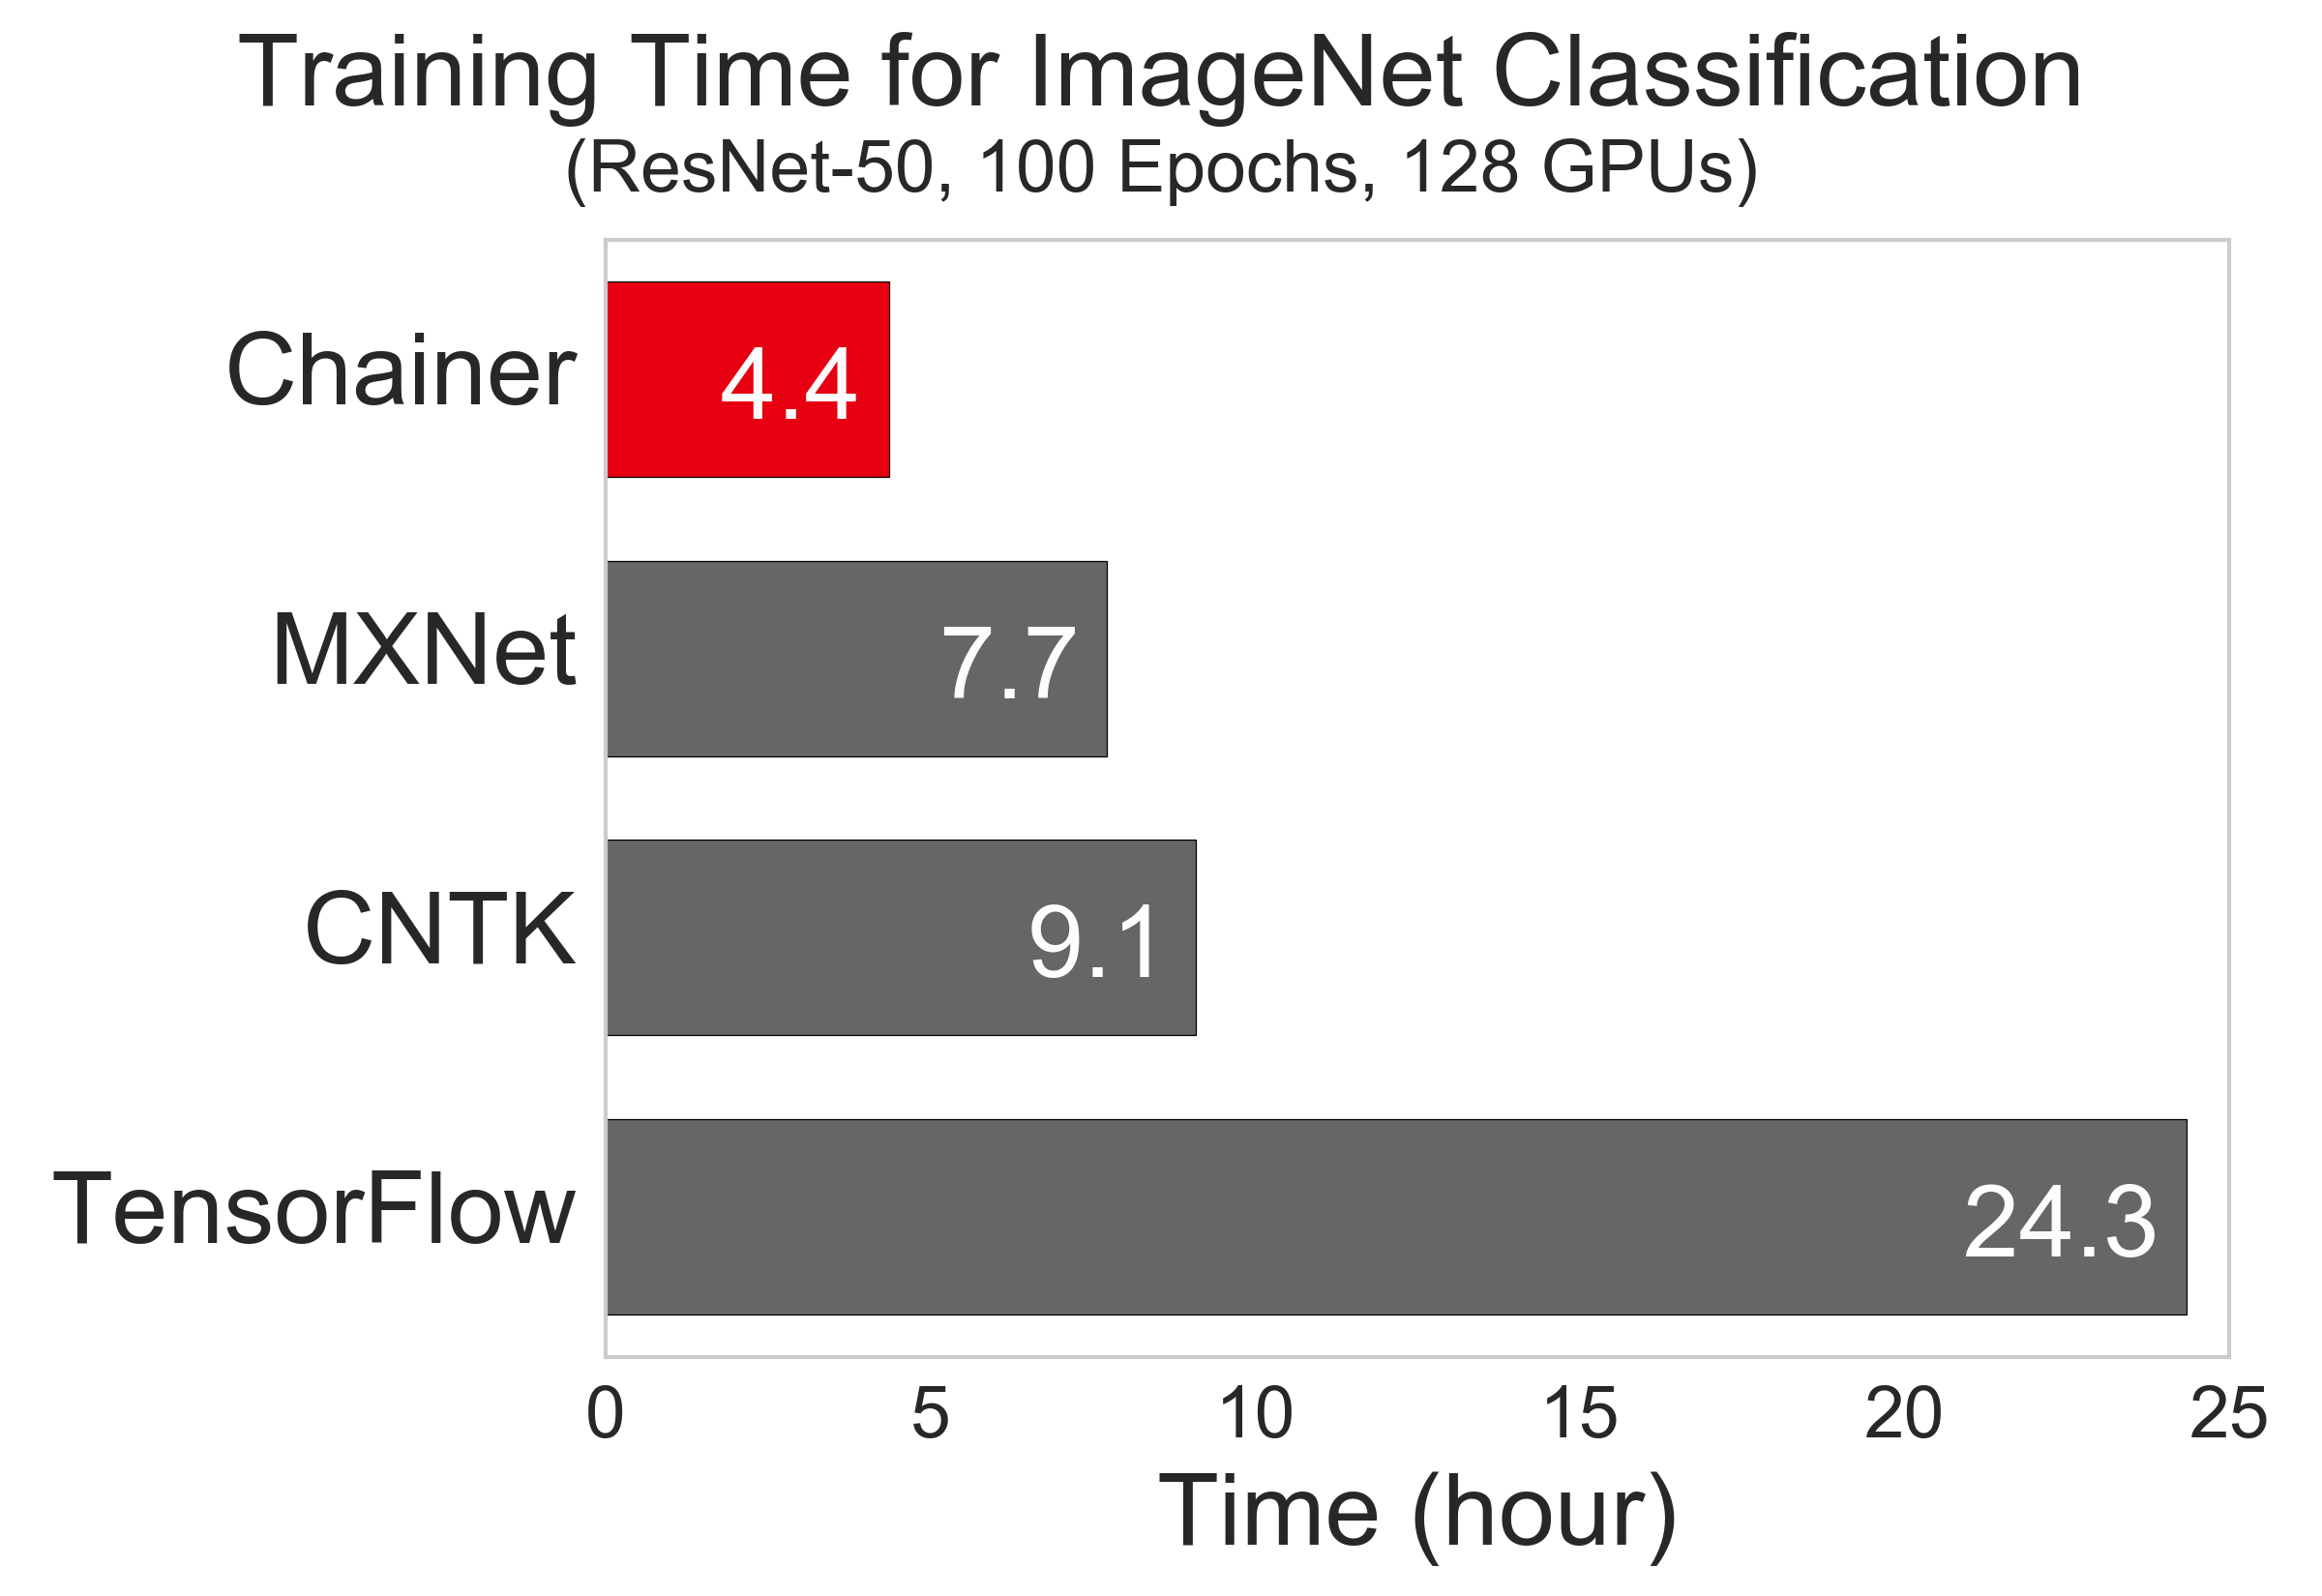
\includegraphics[width=0.9\linewidth]{Pictures/Chainer_Comparisson}
	\caption[Deep Learning Framework Vergleich]{Deep Learning Framework Vergleich \cite{Chainer}}
	\label{fig:chainercomparisson}
\end{figure}

\subsection{\acf{cntk}}
\ac{cntk} ist ein Open-Source Framework für das verteilen einer Deep-Learning Anwendung im kommerziellen Bereich. Es beschreibt neuronale Netze als eine Reihe von Rechenschritten über einen gerichteten Graphen. \ac{cntk} erlaubt dem Benutzer, populäre Modelltypen wie feed-forward DNNs, konvolutionelle neurale Netze (CNNs) und wiederkehrende neurale Netze (RNNs / LSTMs) leicht zu verwirklichen und zu kombinieren. \ac{cntk} implementiert stochastisches Gradientenabstiegsverfahren (SGD, Error Backpropagation) mit automatischer Differenzierung und Parallelisierung über mehrere \ac{gpu}s und Server hinweg \cite{CNTK}.

\subsection{Apache MXNet}
Apache MXNet ist ein modernes Open-Source Deep Learning Framework, mit dem neuronale Netze trainiert werden können. Es ist skalierbar, ermöglicht schnelles Modelltraining und unterstützt ein flexibles Programmiermodell und mehrere Programmiersprachen. Die MXNet-Bibliothek ist portabel und kann auf mehreren \ac{gpu}s und mehreren Instanzen skaliert werden. MXNet wird von den wichtigsten Public Cloud-Anbietern wie \ac{aws} und Azure unterstützt \cite{WikipediaApacheMXNet}. Amazon und Microsoft arbeiteten zusammen an einer \ac{api} für Apache MXNet und veröffentlichten im Oktober 2017 Gluon, eine neue Open-Source Deep-Learning Schnittstelle, die es Entwicklern ermöglicht, einfach und schnell Machine-Learning-Modelle zu erstellen, ohne dabei die Leistung zu beeinträchtigen \cite{AWSintroducingGluon}.

\subsection{Amazon \acs{dsstne}}
Amazon \ac{dsstne} ist eine Open-Source Deep Learning Framework zum entwicklen von Empfehlungsmodellen. \ac{dsstne} wurde bei Amazon eingesetzt, um personalisierte Produktempfehlungen für ihre Kunden zu erstellen. Es ist für den produktiven Einsatz von realen Anwendungen ausgelegt, bei denen Geschwindigkeit und Skalierbarkeit gegenüber experimenteller Flexibilität im Vordergrund stehen müssen. Training und Vorhersagen werden skaliert, wobei Berechnung und Speicherung für jede Schicht modellparallel verteilt werden \cite{Amazon DSSTNE}.

\subsection{Eclipse \acl{dl4j}}
Eclipse \ac{dl4j} ist die erste kommerzielle, Open-Source, verteilte Deep-Learning-Bibliothek für Java und Scala. Durch die Integration mit Hadoop und Apache Spark bringt \ac{dl4j} \ac{ki} vor allem zu Geschäftsumgebungen bei der diese Technologien bereits im Einsatz sind. \ac{dl4j} zielt darauf ab, Plug-and-Play auf dem neuesten Stand der Technik zu sein, mehr Konvention als Konfiguration. Dies ermöglicht ein schnelles Prototyping für Data Scientists, Machine-Learning-Praktiker und Softwareentwickler. \ac{dl4j} ist im Maßstab anpassbar. Unter der Apache 2.0-Lizenz veröffentlicht, gehören alle Derivate von \ac{dl4j} ihren Autoren. \ac{dl4j} kann Modelle aus Frameworks wie TensorFlow, Caffe und Theano importieren \cite{dl4j}. \newline

Wie zu sehen, gibt es aktuell viele Deep Learning Frameworks. Die meisten dieser Framework sind Open-Source Projekte und auf GitHub veröffentlicht. Heutzutage ist es wichtig, dass sich diese Technologie schnell weiterentwickeln, dazu ist eine große Gemeinschaft an Entwicklern notwendig. Abbildung \ref{fig:githubinterestdeeplearning} zeigt das Interesse dieser Gemeinschaft an den verschiedenen Deep Learning Frameworks vom 1. Juli 2018. Das Framework TensorFlow wird dabei besonders viel Interesse geschenkt, deshalb wollen wir dieses Framework im nächsten Kapitel genauer untersuchen.

\begin{figure}
	\centering
	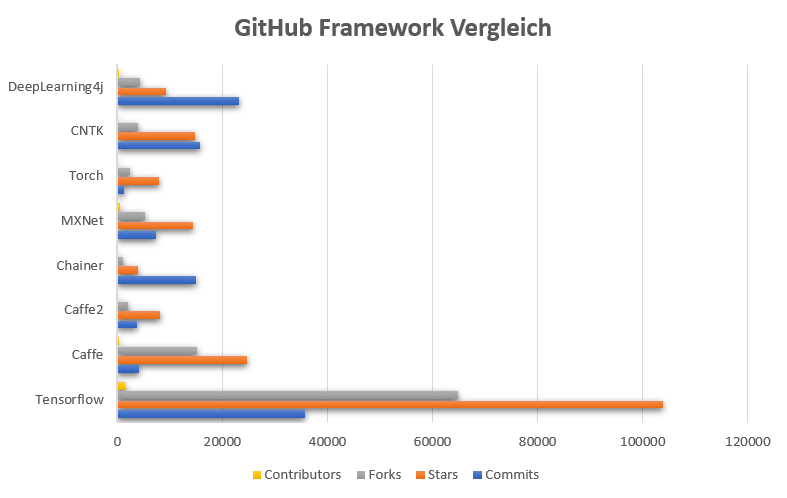
\includegraphics[width=0.9\linewidth]{Pictures/GitHubFrameworkVergleich}
	\caption[GitHub: Vergleich des Interesses in verschiedene Deep Learning Frameworks]{GitHub: Vergleich des Interesses an o.g. Deep Learning Frameworks}
	\label{fig:githubinterestdeeplearning}
\end{figure}

\section{TensorFlow}\label{sec:tensorflow}
TensorFlow ist eine Open-Source-Softwarebibliothek für die numerische Hochleistungsberechnung. Die flexible Architektur ermöglicht die einfache Implementierung von Berechnungen auf einer Vielzahl von Plattformen (\ac{cpu}s, \ac{gpu}s, TPUs) und von Desktops über Cluster von Servern bis hin zu mobilen und Edge-Geräten. Ursprünglich von Forschern und Ingenieuren des Google Brain-Teams in der KI-Organisation von Google entwickelt, bietet es eine starke Unterstützung für maschinelles Lernen und Deep Learning. Der Kern der flexiblen numerischen Berechnung wird in vielen anderen wissenschaftlichen Bereichen eingesetzt \cite{tensorflow}.

\subsection{Installation}
TensorFlow kann auf den folgenden Plattformversionen und höher installiert werden: 
\begin{itemize}
	\item macOS 10.12.6 
	\item Ubuntu 16.04 
	\item Windows 7 
\end{itemize}

Standardmäßig werden Anwendungen für TensorFlow in der Programmiersprache Python geschrieben, es lassen sich jedoch Entwicklungsumgebungen für die Programmiersprachen C++, Go, Swift und Java einrichten.

\subsection{Unterstützung von mobilen Plattformen}
Google stellt verschiedene Versionen ihres Frameworks bereit. Unter anderem auch Versionen für mobile Endgeräte, die für diese optimiert sind und mit weniger zur Verfügung stehenden Ressourcen auskommen. Im folgenden werden die verschiedenen Versionen kurz vorgestellt.

\subsubsection{TensorFlow Mobil}
TensorFlow Mobil wurde für den Einsatz auf einem mobilen Gerät optimiert und enthält alle Funktionen die das Framework zu bieten hat. Jedoch bietet TensorFlow Mobil nicht die optimale Performance für mobile Geräte. Deshalb wurde TensorFlow Light entwickelt, welches sich aktuell noch im Entwicklungsstatus befindet. Dabei werden von TensorFlow Light nur eine begrenzte Anzahl an Funktionen unterstützt, sodass die binäre Größe kleiner ist und damit ein Performance-Steigerung erzielt werden kann. Ob TensorFlow Mobil oder Light für eine Anwendung eingesetzt wird, hängt von deren Anforderungen ab \cite{tensorflow}. 

\subsubsection{TensorFlow Light}
TensorFlow Lite ist eine Lösung für mobile und eingebettete Geräte wie beispielsweise Smartphones oder Smartwatches. Es ermöglicht maschinelles Lernen auf dem Gerät mit geringer Wartezeit und einer kleinen binären Größe. TensorFlow Lite unterstützt auch Hardware-Beschleunigung mit der Android Neural Networks \ac{api}. TensorFlow Lite verwendet viele Techniken, um niedrige Latenzzeiten zu erreichen, wie z. B. die Optimierung der Kernel für mobile Apps, vorfusionierte Aktivierungen und quantisierte Kernel, die kleinere und schnellere Modelle ermöglichen \cite{tensorflow}. Gerade der Einsatz von einem Deep Learning Framework direkt auf einem mobilen Gerät ermöglicht viele neue Anwendungsfälle und erlaubt auch den Einsatz des Frameworks, wenn das mobile Gerät keine Internetverbindung hat. Meist reicht es auch aus, wenn auf dem mobilen Gerät ein bereits trainiertes Modell genutzt wird, sofern kein weiteres Training des Modells nötig ist. 

\subsubsection{TensorFlow.js}
TensorFlow.js ist eine JavaScript-Bibliothek zum Trainieren und Bereitstellen von Machine Learning Modellen im Browser und auf Node.js. Es können entweder vorhandene Modelle genutzt und weiter trainiert oder neue Modelle mit einer innovativen \ac{api} gebaut und bereitgestellt werden \cite{tensorflowjs}. Dies ermöglicht die Integration von maschinellem Lernen in Webseite, die auf jeder Plattform mit einem Browser genutzt werden kann.


\section{Verteiltes TensorFlow}
Nachdem im vorherigen Kapitel einen kleiner Überblick über TensorFlow gegeben wurde, soll jetzt die Verteilung einer TensorFlow Umgebung auf mehrere Instanzen näher betrachtet werden. Dieses Kapitel stellt nötiges Wissen bereit, dass im nächsten Kapitel im Rahmen eines Tutorials zur Einrichtung einer verteilten TensorFlow Umgebung eingesetzt wird. 

\subsection{Architektur}
Im folgenden wird die Architektur einer verteilten TensorFlow Umgebung genauer beschrieben. Dabei wird zwischen dem Parameterserver und Arbeiter unterschieden.

\subsubsection{Parameterserver}
Der Parameterserver verwaltet das aktuelle Model mit seinen Gewichtungen und Variablen und verteilt es an die Arbeiter. Falls durch mehrere Arbeiter zu viel Ein-/Ausgabe Anfragen an den Parameterserver erzeugt werden, können mehrere Parameterserver eingesetzt werden, um die Last zu verteilen. Mehreren Parameterserver synchronisieren das Model untereinander. Abbildung \ref{fig:architektur-servemodel} zeigt, wie das Verteilen des Models an die Arbeiter aussehen kann. 

\begin{figure}[h!]
	\centering
	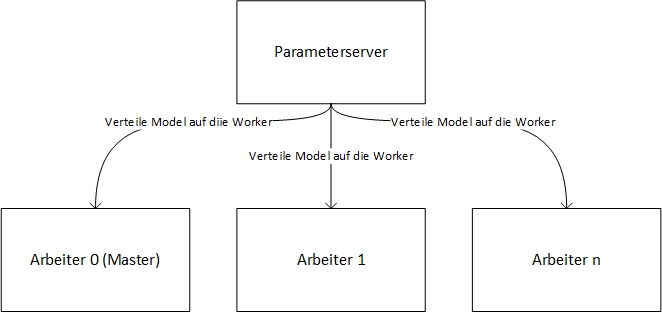
\includegraphics[width=0.9\linewidth]{Pictures/Architektur-ServeModel}
	\caption[Verteilen des Models auf die Arbeiter]{Verteilen des Models auf die Arbeiter}
	\label{fig:architektur-servemodel}
\end{figure}

\subsubsection{Arbeiter}
Arbeiter führen ressourcenintensive Berechnung durch zur Optimierung des vom Parameterserver bereitgestellten Models. Nach der Optimierung sendet der Arbeiter das neue Model mit seinen Gewichtungen und Variablen zum Parameterserver. Desto mehr Arbeiter eingesetzt werden, desto schneller und effizienter kann ein Model trainiert werden. Abbildung \ref{fig:architektur-updatemodel} zeigt, wie die Berechnung des Models und die Aktualisierung des Models auf dem Parameterserver aussehen kann. Der Master Arbeiter koordiniert die Trainingsvorgänge und kümmert sich um die Initialisierung des Modells, Zählen der Anzahl der ausgeführten Trainingsschritte, Speichern und Wiederherstellen von Modellkontrollpunkten.

\begin{figure}[h!]
	\centering
	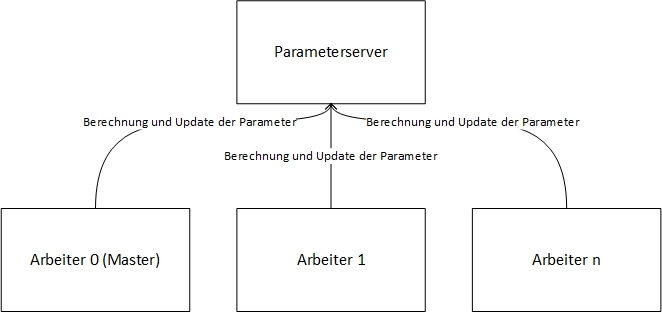
\includegraphics[width=0.9\linewidth]{Pictures/Architektur-UpdateModel}
	\caption[Berechnung des Models auf Arbeiter + Updaten der Variablen auf dem Parameterserver]{Berechnung des Models auf Arbeiter + Updaten der Variablen auf dem Parameterserver}
	\label{fig:architektur-servemodel}
\end{figure}

\subsection{Datenparallelität}
Es gibt zwei verschiedene Möglichkeiten für Datenparallelität:
\subsubsection{Synchron}
Die Arbeiter lesen gleichzeitig das Model vom Parameterserver und berechnen mit diesem ihre Trainingsoperationen und warten, bis die anderen Arbeiter fertig sind. Dann werden die Ergebnisse gemittelt und eine Aktualisierung des Models wird an den Parameterserver gesendet. Somit hat zu jedem Zeitpunkt jeder Arbeiter das gleiche Model.

\subsubsection{Asynchron}
Die Arbeiter lesen asynchron von den Parameterserver, berechnen ihre Trainingsoperation und senden asynchrone Aktualisierungen an den Parameterserver. Zu jedem Zeitpunkt könnten zwei verschiedene Arbeiter unterschiedliche Werte für ihr Model besitzen.

\subsection{Weitere Möglichkeiten}
Bisher wurde die einfachste Methode beschrieben, wie ein verteilte TensorFlow Umgebung eingerichtet werden kann. Es gibt auch die Möglichkeit eine verteilte TensorFlow Umgebung auf Basis von Hadoop \cite{tensorflowhadoop}, Kubernetes \cite{tensorflowkubernetes}, Docker \cite{tensorflowdocker} und Apache Spark \cite{tensorflowspark} zu erstellen.





\section{Tutorial: Erstellung einer verteilten TensorFlow Umgebung}
Nachdem im vorherigen Kapitel das Konzept einer verteilten TensorFlow Umgebung erläutert wurde, wollen wir Schritt für Schritt eine solche Umgebung einrichten.

\subsection{Vorbereitung der Instanzen}
Als erstes müssen wir vier Instanzen aufsetzten. Wenn möglich sollte jede Instanz die gleichen Ressourcen zur Verfügung haben. In meinem Fall habe ich vier virtuelle Maschinen in der StudiCloud der Hochschule Furtwangen erstellt. Jede virtuelle Maschine hat eine virtuelle \ac{cpu}, 1GB RAM und 10GB Festplattenspeicher zur Verfügung. Auf den virtuellen Maschinen wurde Ubuntu Server 16.04 installiert. Um die Kommunikation unter den virtuellen Maschinen zu vereinfachen, setzten wir wie in Abbildung \ref{fig:hostkonfiguration} für jede virtuelle Maschine einen Hostname und die anderen virtuellen Maschinen als Hosts. 

\begin{figure}[h!]
	\centering
	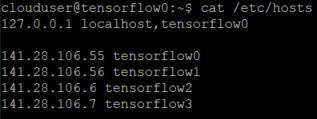
\includegraphics[width=0.9\linewidth]{Pictures/HostKonfiguration}
	\caption[Hosts Konfiguration]{Exemplarische Hosts Konfiguration}
	\label{fig:hostkonfiguration}
\end{figure}

Im Idealfall sollten Instanzen mit wesentlich mehr \ac{cpu} Leistung und einer zusätzlichen Grafikkarte eingesetzt werden, nur somit ist eine optimale Performance möglich. Im Rahmen dieser Arbeit standen mir diese Mittel nicht zur Verfügung.

\subsection{Installation von TensorFlow}
Nun müssen wir auf den virtuellen Maschinen Python und TensorFlow installieren. Python benötigen wir zum Entwickeln unserer Beispielanwendung und wir nutzen Python's Paketmanager pip zur Installation von TensorFlow. Dazu müssen folgende Befehle auf den virtuellen Maschinen ausgeführt werden.
\begin{itemize}
	\item Installation von Python zur Entwicklung:\newline
			\texttt{sudo apt-get install python3-dev}
	\item Installation von Python's Paketmanager pip\newline
			\texttt{sudo apt-get install python3-pip}
	\item Installation von TensorFlow via pip\newline
			\texttt{pip3 install tensorflow}
\end{itemize}

\subsection{Entwicklung einer Anwendung}
Unsere virtuellen Maschinen mit einer Python- und TensorFlow Installation sind jetzt Einsatzbereit. Jetzt wollen wir eine einfache TensorFlow Anwendung erstellen, die eine virtuelle Maschine als Parameterserver und zwei virtuelle Maschinen als Arbeiter nutzt. Wir entwickeln die Anwendung lokal auf unserem Computer und verteilen sie danach auf die virtuelle Maschinen. Dazu erstellen wir die Datei \textit{"train.py"} und öffnen sie in einer Entwicklungsumgebung unser Wahl (in meinem Fall Visual Studio Code). 

\vspace{2mm}
\subsubsection{Erstellung eines Clusters}
Als erstes müssen wir ein Cluster aus Arbeiter und Parameterserver Instanzen definieren. Diese werden bei Anwendungsstart in den Argumenten "\textit{--worker\_hosts}" und "\textit{--ps\_hosts}" übergeben. Dies bietet den Vorteil, dass wir die gleiche Anwendung für Arbeiter bzw. Parameterserver verwenden können.

\begin{itemize}
	\item Parsen der Argumenten: \newline
		\texttt{ps\_hosts = FLAGS.ps\_hosts.split(",")} \newline
		\texttt{ps\_hosts = FLAGS.ps\_hosts.split(",")}
	\item Erstellung des Clusters mit den Arbeitern und Parameterservern anhand der Parameter: \newline
			\texttt{cluster = tf.train.ClusterSpec({"ps": ps\_hosts, "worker": worker\_hosts})}
\end{itemize}

\vspace{2mm}
\subsubsection{Starten der Instanz}
Nachdem wir ein Cluster erstellt haben, müssen wir die jeweilige Instanz starten, dazu nutzen wir die Argumente "\textit{--job\_name}" und "\textit{--task\_index}".
\begin{itemize}
	\item Starten der Instanz: \newline
		\texttt{server = tf.train.Server(cluster,
				job\_name=FLAGS.job\_name,	
				task\_index=FLAGS.task\_index)}
\end{itemize}

\vspace{2mm}
\subsubsection{Parameterserver}
Als nächstes müssen wir schauen, ob die aktuelle Instanz als Arbeiter oder Parameterserver dienen soll. Wenn die Instanz als Parameterserver dient, soll sie keine Berechnung durchführen, sondern warten bis ein Arbeiter Attribute anfordert oder aktualisieren will.
\begin{itemize}
	\item Initialisierung einer Instanz als Parameterserver: \newline
		\texttt{if FLAGS.job\_name == 'ps': 
			server.join()}
\end{itemize}

\vspace{2mm}
\subsubsection{Arbeiter}
Wenn eine Instanz kein Parameterserver ist, ist sie automatisch ein Arbeiter und führt Berechnungen durch. Die Arbeiter führen ihre Berechnungen synchron durch und warten deshalb nach jeder Iteration, bis jeder Arbeiter die Variablen auf dem Parameterserver synchronisiert hat. Anschließend verteilt der Parameterserver wieder die aktualisierten Variablen an die Arbeiter. Wir wollen dabei nicht genauer auf die Berechnungen eingehen und nutzen daher einen Beispielcode eines Tutorials von TensorFlow und schauen uns an, wie die eine Berechnung auf einem Arbeiter durchgeführt wird:

\begin{itemize}
	\item Zuweisung einer Berechnung zu einem Arbeiter: \newline
		\texttt{with tf.device(tf.train \newline
			\hspace*{5mm} .replica\_device\_setter(
			\hspace*{5mm} worker\_device="/job:worker/task:\%d",\newline
			\hspace*{5mm} \% FLAGS.task\_index, cluster=cluster)):}
	\item Parsen des Arguments "is\_chief", welches angibt, ob ein Arbeiter als Master fungiert: \newline
		\texttt{is\_chief = (FLAGS.task\_index == 0)}
	\item Starten einer neuen Session auf einem Arbeiter: \newline
		\texttt{sess = tf.train.MonitoredTrainingSession(
			master=server.target,
			is\_chief=is\_chief)}
	\item Starten einer Berechnung in der Session: \newline
		\texttt{sess.run(task)}
	\item Beenden einer Session, sobald die Berechnung beendet wurde: \newline
		\texttt{sess.close()}
\end{itemize}

Nun haben wir alle wichtigen Konfiguration für unsere verteilte TensorFlow Umgebung vorgenommen. Der komplette Quellcode der Beispielanwendung kann unter "https://github.com/MichZipp/Exploring-Distributed-Tensorflow/Code" gefunden werden. 

\subsection{Starten einer Anwendung}
Jetzt müssen wir die Anwendung noch starten, dazu müssen wir zuerst unsere \textit{"train.py"} mit dem \ac{ftp} auf unsere Instanzen kopieren. Als nächstes müssen wir die Anwendung auf jeder Instanz mit den richtigen Argumenten starten. Um diesen Prozess zu vereinfachen, schreiben wir uns ein kleines Bash-Skript, dass wir dann nur auf dem Master Arbeiter starten müssen:

\begin{itemize}
	\item Bash-Script \textit{"run.sh"} für ein Cluster aus zwei Arbeitern und einem Parameterserver: \newline
		\texttt{\#!/bin/bash \newline
			ssh clouduser@tensorflow2 \newline
			\hspace*{5mm} 'python3 ~/Tensorflow/trainer.py \newline
			\hspace*{5mm} --ps\_hosts="tensorflow2:2222" \newline
			\hspace*{5mm} --worker\_hosts="tensorflow0:2222, \newline 
			\hspace*{10mm} tensorflow1:2222" \newline
			\hspace*{5mm} --job\_name="ps" --task\_index=0' \newline
			ssh clouduser@tensorflow1 \newline
			\hspace*{5mm} 'python3 ~/Tensorflow/trainer.py \newline
			\hspace*{5mm} --ps\_hosts="tensorflow2:2222" \newline
			\hspace*{5mm} --worker\_hosts="tensorflow0:2222, \newline
			\hspace*{10mm} tensorflow1:2222" \newline
			\hspace*{5mm} --job\_name="worker" --task\_index=1' \newline
			python3 ~/Tensorflow/trainer.py \newline
			\hspace*{5mm} --ps\_hosts="tensorflow2:2222" \newline
			\hspace*{5mm} --worker\_hosts="tensorflow0:2222, \newline
			\hspace*{10mm} tensorflow1:2222" \newline
			\hspace*{5mm} --job\_name="worker" --task\_index=0}
	\item Ausführen des Bash-Skripts: \newline
		\texttt{bash run.sh}
\end{itemize}

\vspace{2mm}
Um die Cluster-Zusammenstellungen zu verändern, muss nur das Bash-Skript angepasst werden. Bei vier Instanzen können folgende Cluster-Zusammenstellungen verwendet werden:

\begin{itemize}
	\item 1 Arbeiter, 1 Parameterserver
	\item 2 Arbeiter, 1 Parameterserver
	\item 3 Arbeiter, 1 Parameterserver
	\item 1 Arbeiter, 2 Parameterserver
	\item 1 Arbeiter, 3 Parameterserver
	\item 2 Arbeiter, 2 Parameterserver
\end{itemize}

Wie dieses Tutorial zeigt, sind nicht viele Schritte notwendig, um eine verteilte TensorFlow Umgebung einzurichten. 





\section{Evaluierung}
Die Nutzung einer verteilten TensorFlow Umgebung zeigt deutliche Performance Vorteile. Bei der im letzten Kapitel entwickelte Anwendung führen Arbeiter einfache Berechnungen durch und aktualisieren nach jeder Iteration die Variablen auf dem Parameterserver. Bei dieser Anwendung verkürzt sich jedoch die Ausführungszeit nicht, da die Berechnung zu wenig Zeit in Anspruch nimmt und die Anzahl an Iterationen vorgegeben ist. Es ist aber zu sehen, dass wenn mehr als ein Arbeiter eingesetzt wird, sich mit jedem zusätzlichen Arbeiter sich das Ergebnis der Berechnung verbessert. D.h. wenn anstatt einem Arbeiter zwei Arbeiter verwendet werden würden, brächten wir pro Arbeiter nur die Hälfte an Iteration und somit halbe Zeit um das selbe Ergebnis zu erhalten.  
\section{Zusammenfassung}
 Eine \ac{ki} benötigt viel Ressourcen, um eine gute Performance zu gewährleisten. Es gibt heutzutage einige Deep Learning Frameworks, mit der eine \ac{ki} implementiert werden kann. Am Anfang des Artikels werden einige Frameworks vorgestellt. Im Detail wird dann auf das Framework TensorFlow von
 Google eingegangen, dabei werden die unterstützen Plattformversionen und Möglichkeiten, wie TensorFlow auf einem mobilen Endgerät eingesetzt werden kann, beschrieben. Meist reicht eine Instanz nicht aus, um die Anforderungen einer Anwendungen zu erfüllen. Deshalb gibt es die Möglichkeit, mehrere Instanzen zu nutzen, um die Performance des Frameworks zu verbessern. Dazu wird zuerst eine Wissensgrundlage geschaffen, indem die Architektur einer verteilten TensorFlow Umgebung aufgezeigt wird. Anschließend wir erläutert, welche Rolle dabei ein Arbeiter und Parameterserver spielt. Anhand eines Tutorials werden die wichtigsten Schritte für das Aufsetzten einer solchen Umgebung beschrieben, wobei eine kleine Beispielanwendung entwickelt wurde. Diese wurde genutzt, um eine Evaluierung durchzuführen, welche bestätigt, dass der Einsatz von mehreren
 Arbeitern die Performance des Frameworks deutlich verbessert. Dabei wurden verschiedene Konfiguration, unterschiedliche Anzahl an Arbeiter und Parameterserver, für die TensorFlow Umgebung genutzt. Die Performance einer \ac{ki} wird auch in Zukunft eine Herausforderung darstellen, denn die Einsatzgebiete werden immer komplexer und breitgefächerter.  

% *** END OF SECTIONS ***---------------------------------------------
% by themselves when using endfloat and the captionsoff option.
\ifCLASSOPTIONcaptionsoff
  \newpage
\fi

\begin{thebibliography}{1}
\bibitem{PlanetWissenKI}
"Planet Wissen - Künstliche Intelligenz"
\url{https://www.planet-wissen.de/technik/computer_und_roboter/kuenstliche_intelligenz/} 
Accessed 20.06.2018

\bibitem{BigDataInsiderDeepLearning}
"Big Data Insider - Maschinelles Lernen und Deep Learning"
\url{https://www.bigdata-insider.de/ki-maschinelles-lernen-und-deep-learning-das-sind-die-unterschiede-a-588067/} 
Accessed 20.06.2018

\bibitem{DeepLearningFrameworks}
"DL4J - Deep Learning Frameworks Comparison"
\url{https://deeplearning4j.org/compare-dl4j-tensorflow-pytorch}
Accessed 20.06.2018

\bibitem{Torch}
"Torch"
\url{https://pytorch.org/about/}
Accessed 20.06.2018

\bibitem{Caffe}
"Caffe"
\url{http://caffe.berkeleyvision.org/}
Accessed 21.06.2018

\bibitem{Caffe2}
"Caffe2"
\url{https://caffe2.ai/}
Accessed 21.06.2018

\bibitem{Keras}
"Keras"
\url{https://keras.io/}
Accessed 24.06.2018

\bibitem{Elephas}
"Elephas"
\url{https://github.com/maxpumperla/elephas}
Accessed 24.06.2018

\bibitem{Chainer}
"Chainer"
\url{https://chainer.org/blog/}
Accessed 01.07.2018

\bibitem{CNTK}
"\acf{cntk}"
\url{https://docs.microsoft.com/de-de/cognitive-toolkit/}
Accessed 01.07.2018

\bibitem{WikipediaApacheMXNet}
"Wikipedia - Apache MXNet"
\url{https://en.wikipedia.org/wiki/Apache_MXNet}
Accessed 01.07.2018

\bibitem{AWSApacheMXNet}
"AWS Apache MXNet"
\url{https://aws.amazon.com/de/mxnet/}
Accessed 01.07.2018

\bibitem{AWSintroducingGluon}
"AWS Introducing Gluon"
\url{https://aws.amazon.com/de/blogs/aws/introducing-gluon-a-new-library-for-machine-learning-from-aws-and-microsoft/}
Accessed 01.07.2018

\bibitem{Amazon DSSTNE}
"Amazon DSSTNE"
\url{https://aws.amazon.com/de/blogs/aws/introducing-gluon-a-new-library-for-machine-learning-from-aws-and-microsoft/}
Accessed 01.07.2018

\bibitem{dl4j}
"Elipse \acf{dl4j}"
\url{https://deeplearning4j.org/i}
Accessed 01.07.2018

\bibitem{tensorflow}
"Tensorflow"
\url{https://www.tensorflow.org/}
Accessed 01.07.2018

\bibitem{tensorflowjs}
"Tensorflow.js"
\url{https://js.tensorflow.org/}
Accessed 03.07.2018

\bibitem{tensorflowhadoop}
"TensorFlow on Hadoop"
\url{https://www.tensorflow.org/deploy/hadoop}
Accessed 06.07.2018

\bibitem{tensorflowkubernetes}
"TensorFlow on Kubernetes"
\url{https://banzaicloud.com/blog/tensorflow-on-k8s/}
Accessed 06.07.2018

\bibitem{tensorflowdocker}
"TensorFlow on Docker"
\url{https://github.com/tensorflow/ecosystem/tree/master/docker}
Accessed 06.07.2018

\bibitem{tensorflowspark}
"TensorFlow on Apache Spark"
\url{https://databricks.com/blog/2016/01/25/deep-learning-with-apache-spark-and-tensorflow.html}
Accessed 06.07.2018

\end{thebibliography}

% biography section
% 
% If you have an EPS/PDF photo (graphicx package needed) extra braces are
% needed around the contents of the optional argument to biography to prevent
% the LaTeX parser from getting confused when it sees the complicated
% \includegraphics command within an optional argument. (You could create
% your own custom macro containing the \includegraphics command to make things
% simpler here.)
%\begin{biography}[{\includegraphics[width=1in,height=1.25in,clip,keepaspectratio]{mshell}}]{Michael Shell}

% You can push biographies down or up by placing
% a \vfill before or after them. The appropriate
% use of \vfill depends on what kind of text is
% on the last page and whether or not the columns
% are being equalized.

%\vfill

% Can be used to pull up biographies so that the bottom of the last one
% is flush with the other column.
%\enlargethispage{-5in}



% that's all folks
\end{document}


